\chapter{Grokking EA}
\label{chap:Tips and Tricks}

In this chapter, we have collected a few of the most important tips and tricks for working productively with EA.
You can of course decide to skip over to the next chapter but we really believe that spending the time to grok EA is necessary for a pleasant modelling experience!

\section{How to lay out elements}

Layout is always an important factor when using a visual language.
A well laid out diagram is easier to understand and by centralizing important elements or clustering related elements, you can actually impart additional information via a well-chosen layout.

\begin{enumerate}
\item[$\blacktriangleright$] To lay out a group of elements select them by drawing a selection box around them (or select them one by one by holding down \texttt{Ctrl} and clicking on each element).
\begin{figure}[htbp]
\begin{center} 
  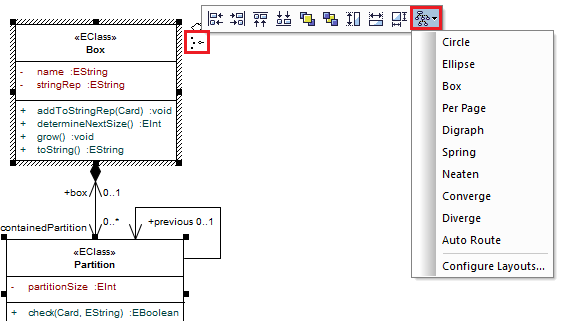
\includegraphics[width=\textwidth]{pics/tricks/layoutElements/layoutElements1}
  \caption{How to layout elements}  
  \label{fig_layout01}
\end{center}
\end{figure}
 
\item[$\blacktriangleright$] At the right side of the element that was selected last, a little symbol appears (Fig.~\ref{fig_layout01}).
Click on the symbol to obtain different options that are applied to all selected elements simultaneously.
Experiment a bit to find out what effect each option has.
The last symbol opens a further drop-down menu with standard layout algorithms.

\begin{figure}[htbp]
\begin{center}  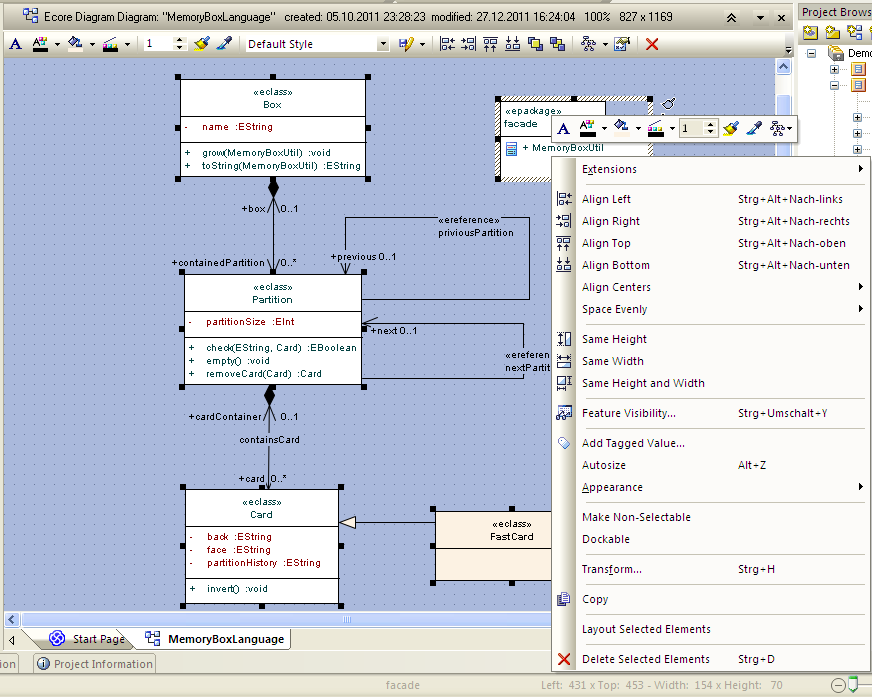
\includegraphics[width=\textwidth]{pics/tricks/layoutElements/layoutElements2}
  \caption{Further layout options}  
  \label{fig_layout02} 
\end{center}
\end{figure}

\item[$\blacktriangleright$] Richt-clicking one of the selected elements opens a different menu with a further set of layout options (Fig.~\ref{fig_layout02}).
Especially \texttt{Align Centers} can be pretty useful.
\end{enumerate}
  
\section{Bending lines to your will}

Almost as important as a good layout is getting lines to be just the way you want them to be.
In EA you can add and remove bending points which can be used to control the appearance of a line.

\begin{enumerate}
\item[$\blacktriangleright$]Hold down \texttt{Ctrl} and click on a line to create a bending point (Fig.~\ref{fig_bendLine01}).
You can now pull and place the bending point as you wish.
 
\begin{figure}[htbp]
\begin{center}
  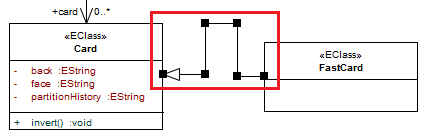
\includegraphics[width=0.8\textwidth]{pics/tricks/bendLine/bendLine1}
  \caption{How to bend lines}   
  \label{fig_bendLine01}
\end{center}
\end{figure}

\item[$\blacktriangleright$] You can create as many bending points as you wish, or \emph{remove} them also by holding down \texttt{Ctrl} and clicking on the point to be deleted.
\end{enumerate}

\section{Deleting vs. removing elements from diagrams}

A central feature that new users should understand as soon as possible is the way EA handles diagrams.
A diagram is simply treated as a \emph{view} of the complete ``model'' in EA.
The complete model can always be browed in a tree view (the package browser) and contains all elements that are exported.
Diagrams typically do not contain all elements and one usually uses multiple possibly ``redundant" diagrams to show different parts of the model.
Thinking in this frame is crucial and provides a pragmatic solution to the problem of having huge unmaintainable diagrams.
A tricky consequence one must get used to is that \emph{removing} an element from a diagram does \emph{not} delete it from the model.

\begin{enumerate}
\item[$\blacktriangleright$] One of the most common mistakes of new users is to remove an element from a diagram by pressing \texttt{Del} and expecting the element to be deleted from the model.   
This is however not the case as the element is only removed from the current diagram and is still in the model and thus in the package browser (Fig.~\ref{fig_DelVsCtrlDel01}).

\begin{figure}[htbp]
\begin{center} 
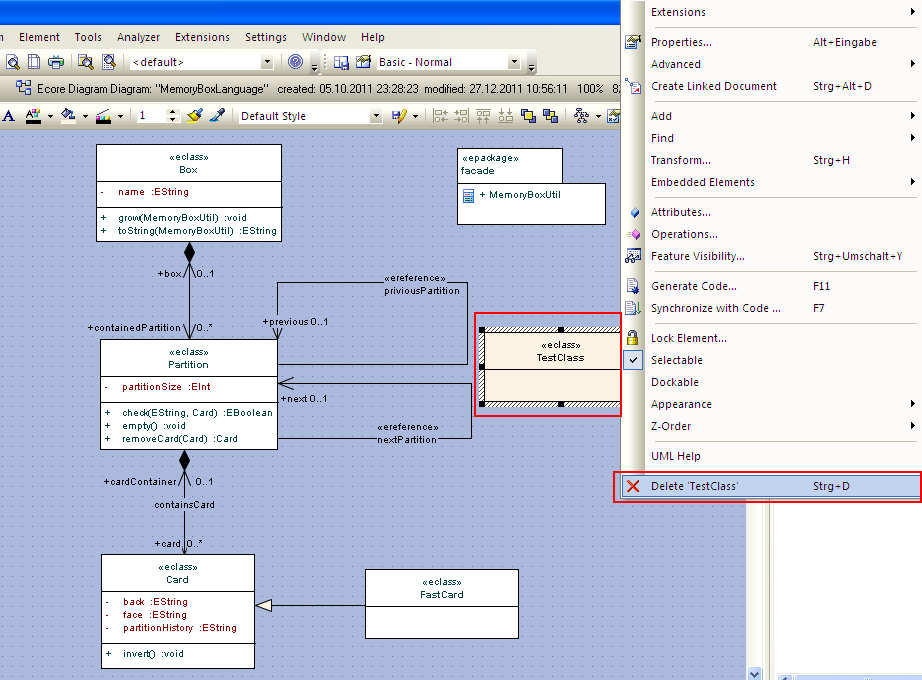
\includegraphics[width=0.87\textwidth]{pics/tricks/DelVsCtrlDel/DelVsCtrlDel1}
  \caption{Removing an element from a diagram via pressing \texttt{Del} does not delete it from the model and it is still present in the package browser}  
    \label{fig_DelVsCtrlDel01}
\end{center}
\end{figure}  

\item[$\blacktriangleright$] By pressing \texttt{Ctrl+Del} and confirming (Fig.~\ref{fig_DelVsCtrlDel02}) you can \emph{delete} an element from a diagram \emph{and} completely from the model as well (the element will no longer be in the \texttt{Project Browser}).
Elements can also be deleted via the context menu in the \texttt{Project Browser} (invoked by right-clicking the element in the \texttt{Project Browser}).

\begin{figure}[htbp]
\begin{center}
  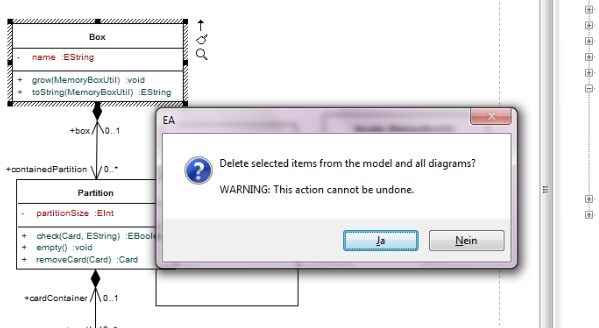
\includegraphics[width=0.7\textwidth]{pics/tricks/DelVsCtrlDel/DelVsCtrlDel2.png}
  \caption{Deleting an element from a diagram and from the model}  
  \label{fig_DelVsCtrlDel02}
\end{center}
\end{figure}  

\end{enumerate}

\section{Excluding certain projects from the export}

Sometimes it might be necessary to be able to exclude projects from the export (\texttt{Export All to Workspace} option).
This might be (i) because the project is still work in progress and simply not yet ready to be exported, (ii) because the complete project is present in your Eclipse workspace but has not been modelled completely in EA and you wish to do this gradually on demand (this is currently the recommended strategy as we do not have an import yet), (iii) because the project is not meant to be present in your Eclipse workspace as generated code and is instead provided via a plugin (this is usually the case for standard metamodels like Ecore, UML etc.), or (iv) because the project is rather large and pretty stable, and you do not want to wait each time for an unnecessary export (and you do not wish to click and export the other projects individually).

Whatever the reason, you can achieve this by setting a certain \emph{tagged value} of the project to be ignored:

\begin{enumerate}
\item[$\blacktriangleright$]Select ``View/Tagged Values'' from the menu bar (Fig.~\ref{fig_ignoreExportingProject01}).
\begin{figure}[htbp]
\begin{center}  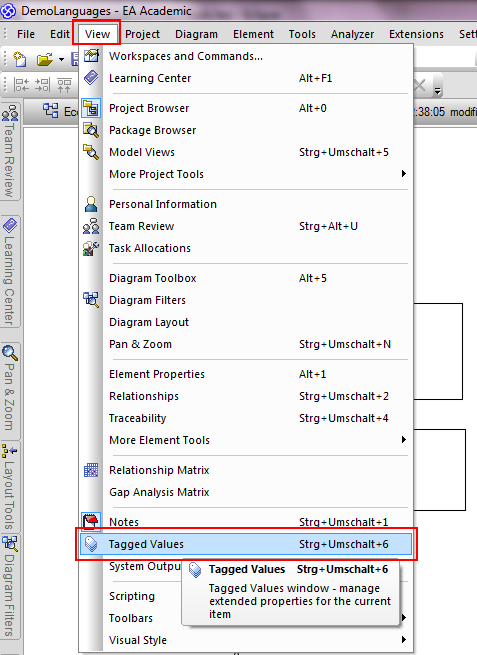
\includegraphics[width=0.55\textwidth]{pics/tricks/ignoreExportingProject/ignoreExportingProject1}
  \caption{view the TaggedValue}  
  \label{fig_ignoreExportingProject01}
\end{center}
\end{figure} 

\item[$\blacktriangleright$] A tagged value \emph{Moflon::Export} should already be present and be set to \texttt{true} per default (Fig.~\ref{fig_ignoreExportingProject02}). 
If this is not the case then create it afresh.
If you want the project to be ignored by the export, change the value of Moflon::Export to \texttt{false} (and conversely back to \texttt{true} to export it again).
\begin{figure}[htbp]
\begin{center}
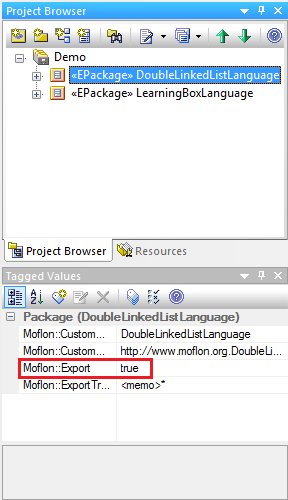
\includegraphics[width=0.5\textwidth]{pics/tricks/ignoreExportingProject/ignoreExportingProject2}
  \caption{Tagged value Moflon::Export is used to ignore projects}  
  \label{fig_ignoreExportingProject02}
\end{center}
\end{figure}
\end{enumerate}


\section{Using Verbose tag to show create and destroy stereotypes} As you have already seen in previous chapters there are different colors in SDMs in 
order to distinguish between ``create'' and ``destroy''.

\begin{enumerate}
\item[$\blacktriangleright$]If you want to have a black white print of diagram 
you can set the these properties in a \emph{verbal} way. Right–click on the
diagram and select'' Extensions/extras/Set Moflon::Verbose to
true''. Now you can see \texttt{<<create>>} and \texttt{<<destroy>>} on the
links (Fig.~\ref{fig_usingVerbose01}).

\begin{figure}[htbp]
\begin{center}
  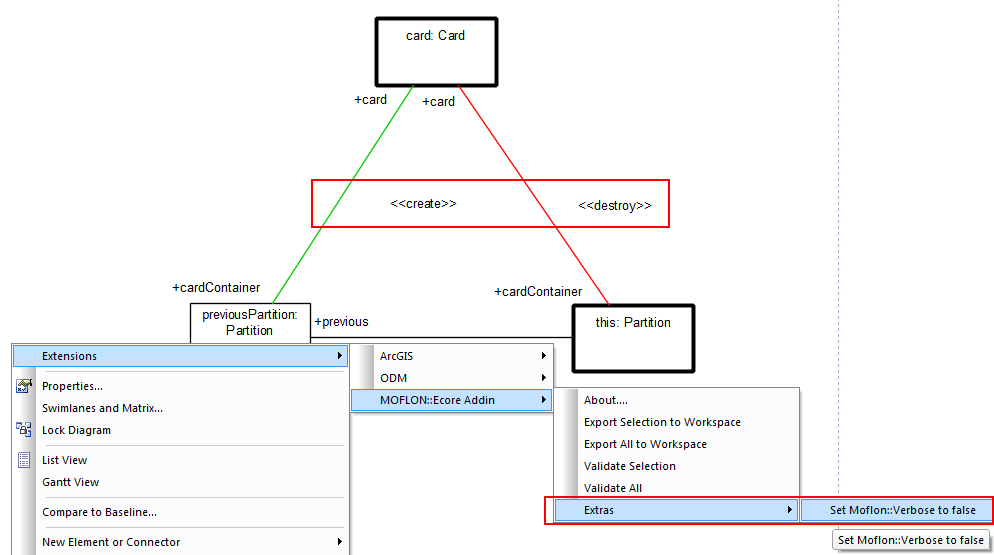
\includegraphics[width=0.5\textwidth]{pics/tricks/usingVerbose/usingVerbose1}
  \caption{Verbal change of links}  
  \label{fig_usingVerbose01}
\end{center}
\end{figure}


\item[$\blacktriangleright$]You can undo this change by selecting
``Extensions/extras/Set Moflon:: Verbose to
false'' (Fig.~\ref{fig_usingVerbose02}).

 \begin{figure}[htbp]
\begin{center}
  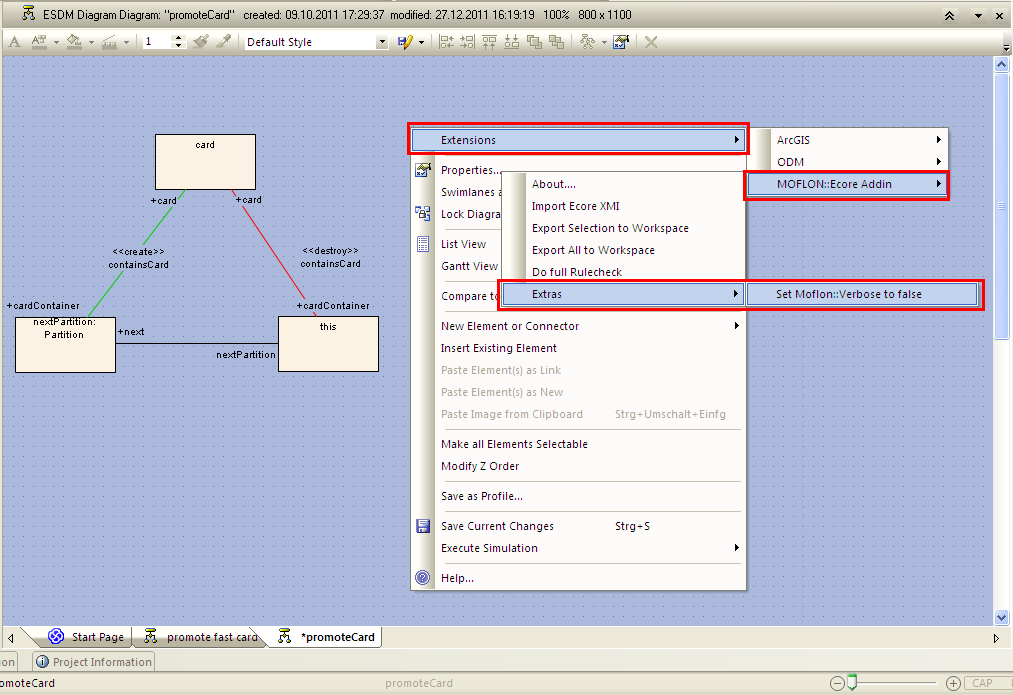
\includegraphics[width=0.5\textwidth]{pics/tricks/usingVerbose/usingVerbose2}
  \caption{Undo Verbal change of a link}  
  \label{fig_usingVerbose02}
\end{center}
\end{figure}

\end{enumerate}


\section{Copying object variables with ctrl + drag}
By holding down \texttt{Ctrl} and dragging the objects, you can copy object
variables (Fig.~\ref{fig_copy01}).You can see the new copied object in Project
Browser (Fig.~\ref{fig_copy02}).

\begin{enumerate}
\item[$\blacktriangleright$]
\begin{figure}[htbp]
\begin{center}
  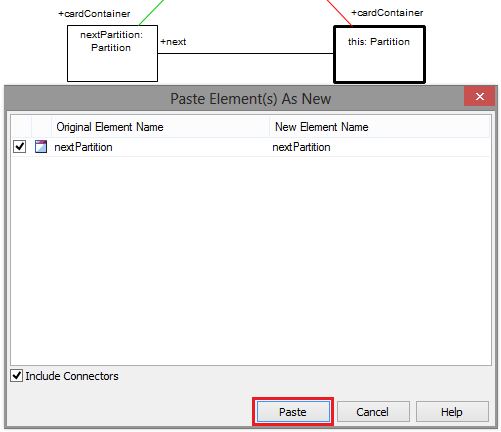
\includegraphics[width=0.5\textwidth]{pics/tricks/copy/copy1}
  \caption{Copying objects}  
  \label{fig_copy01}
\end{center}
\end{figure}


\begin{figure}[htbp]
\begin{center}
  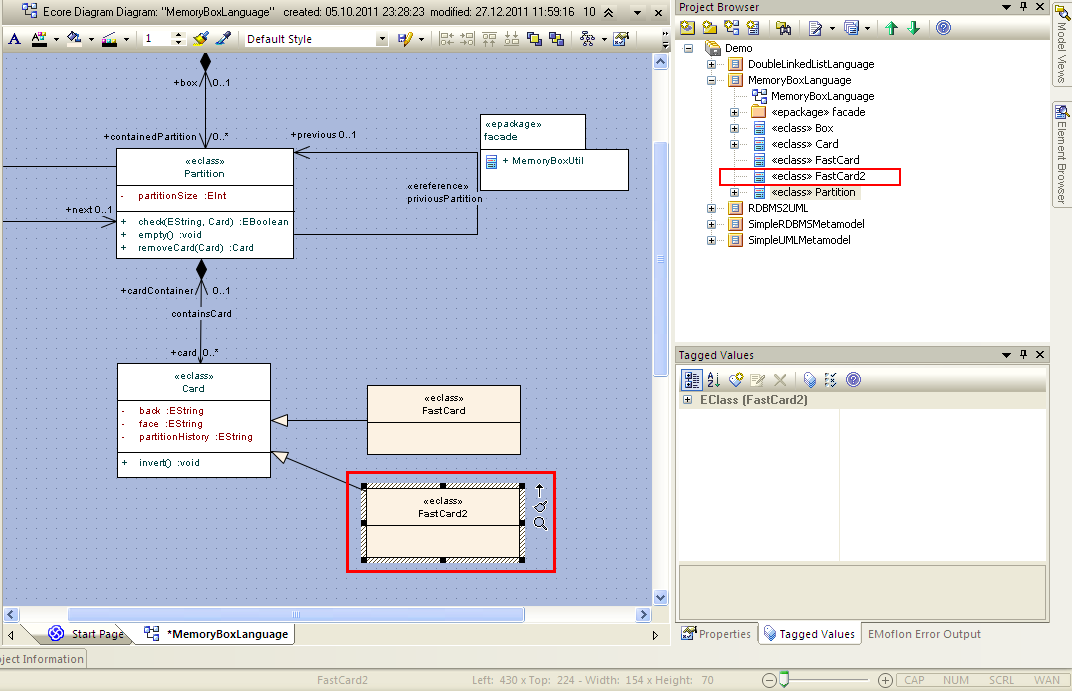
\includegraphics[width=0.5\textwidth]{pics/tricks/copy/copy2}
  \caption{Copied object in Project Browser}  
 
  \label{fig_copy02}
\end{center}
\end{figure}

\end{enumerate}


\section{Searching for Elements}
The Model Search allows you to quickly navigate and find elements within your
model.


\begin{enumerate}
\item[$\blacktriangleright$]Select ``Model Search Window'' and type the name of
element you search for (Fig.~\ref{fig_search01}). 
\begin{figure}[htbp]
\begin{center}
  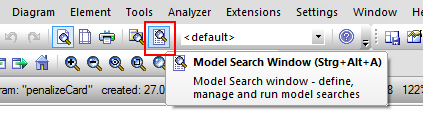
\includegraphics[width=0.5\textwidth]{pics/tricks/search/search1}
  \caption{Model Search Window}  
  \label{fig_search01}
\end{center}
\end{figure}

\item[$\blacktriangleright$]It lists each element that meets the search criteria
you specify within the ``search terms'' and ``search type'' (Fig.~\ref{fig_search02}).
\begin{figure}[htbp]
\begin{center}
  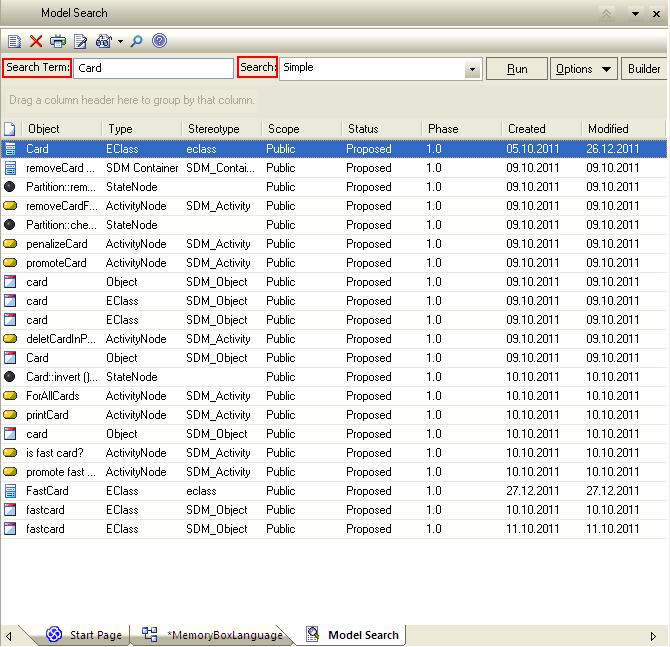
\includegraphics[width=0.5\textwidth]{pics/tricks/search/search2}
  \caption{Enter search criteria}  
  \label{fig_search02}
\end{center}
\end{figure}

\item[$\blacktriangleright$]Right-Click on each of the item and selecting ``Find
in Diagrams'' (Fig.~\ref{fig_search03}). 
\begin{figure}[htbp]
\begin{center}
  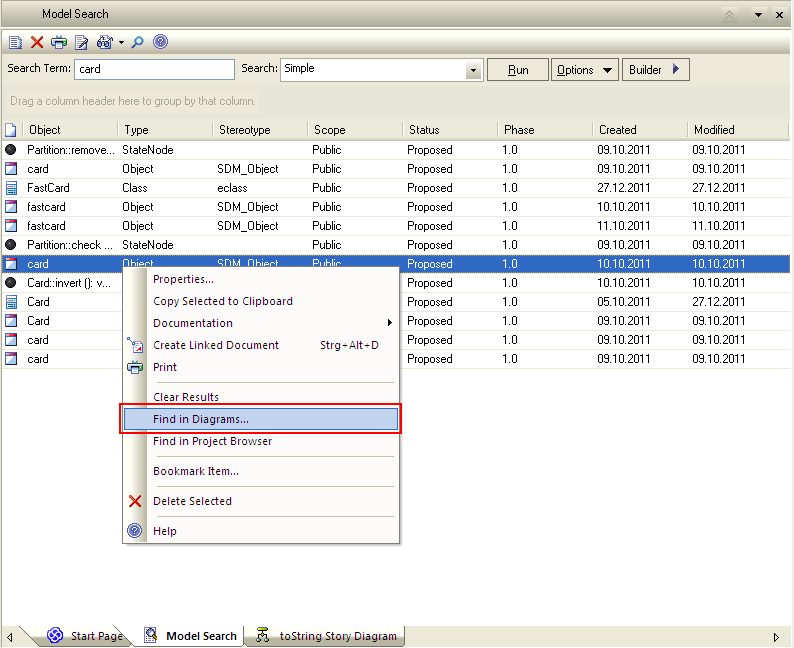
\includegraphics[width=0.5\textwidth]{pics/tricks/search/search3}
  \caption{Finding an element in diagrams}  
  \label{fig_search03}
\end{center}
\end{figure}

\item[$\blacktriangleright$]Right click on each of the item an selecting ``Find in
Project Browser'' (Fig.~\ref{fig_search04}). 
\begin{figure}[htbp]
\begin{center}
  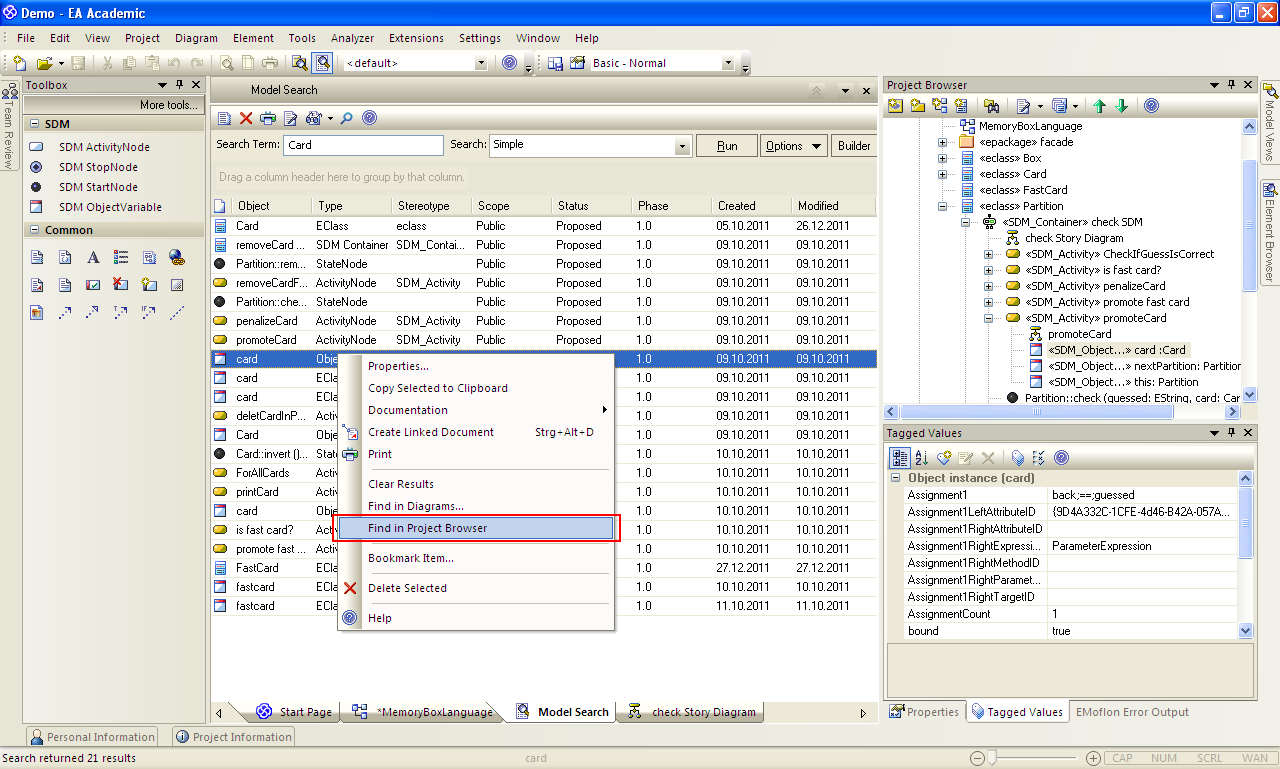
\includegraphics[width=0.5\textwidth]{pics/tricks/search/search4}
  \caption{Finding an element in Project Browser}  
  \label{fig_search04}
\end{center}
\end{figure}

\item[$\blacktriangleright$]If you want to see an specified obejct of a diagram
in the \texttt{Project Browser} , Rightclick on the object and select ``Find/In Project
Browser'' (Fig.~\ref{fig_search05}). In a similar way you can find the
corresponding class of object by Rightclick and selecting ``Find/Locate
Classifier in Project Browser'' (Fig.~\ref{fig_search06}).

\begin{figure}[htbp]
\begin{center}
  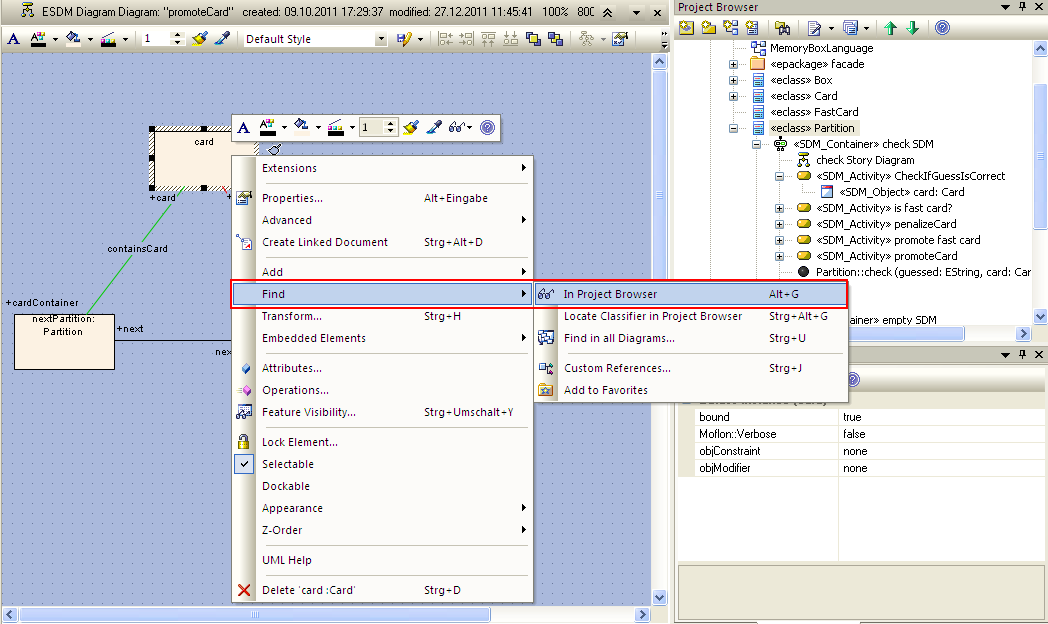
\includegraphics[width=0.5\textwidth]{pics/tricks/search/search5}
  \caption{Following an object from diagram to Projet Browser}  
  \label{fig_search05}
\end{center}
\end{figure}


\begin{figure}[htbp]
\begin{center}
  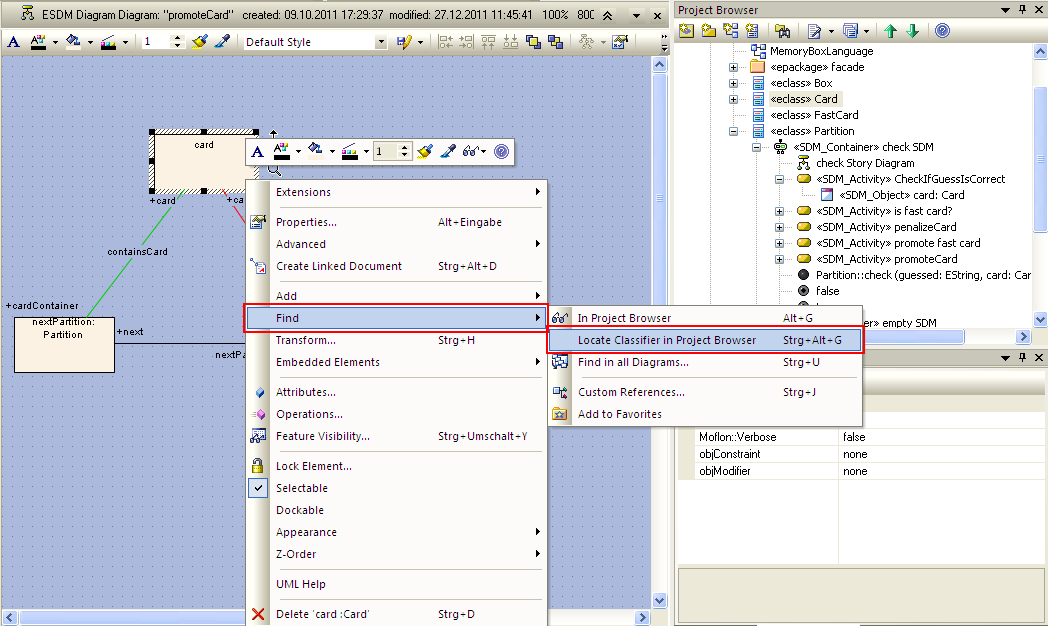
\includegraphics[width=0.5\textwidth]{pics/tricks/search/search6}
  \caption{Finding the corresponding class of an object in the diagram}  
  \label{fig_search06}
\end{center}
\end{figure}

\end{enumerate}


\section{Using multiple EAPs and migrating packages} 

\begin{enumerate}
\item[$\blacktriangleright$]If you want to migrate multiple packages between
multiple EAPs (EA Projects),You can't do it by just copy and
paste the selected packages (Fig.~\ref{fig_projectMigration00}) from/to EAPs.


\begin{figure}[htbp]
\begin{center}
  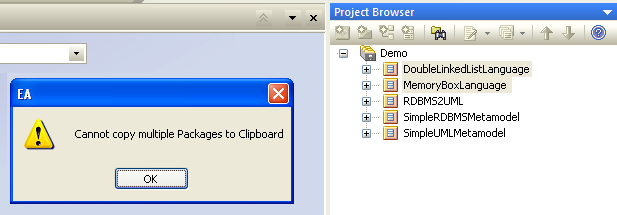
\includegraphics[width=0.5\textwidth]{pics/tricks/projectMigration/projectMigration0}
  \caption{Error message}  
  \label{fig_projectMigration00}
\end{center}
\end{figure}

\item[$\blacktriangleright$]In order to migrate multiple packages, you have to
first export the Whole model(the root node) from one EAP. Right-Click on the root
and select ``Export Model to XMI...''. In the dialogue that
pops up (Fig.~\ref{fig_projectMigration01}), enter the name and path of to be
exported file, choose \texttt{XMI 2.1} as``Export
type'' (Fig.~\ref{fig_projectMigration02}).


\begin{figure}[htbp]
\begin{center}
  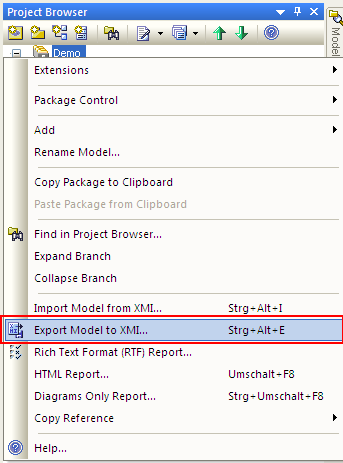
\includegraphics[width=0.5\textwidth]{pics/tricks/projectMigration/projectMigration1}
  \caption{Export the Root Model from the first EAP}  
  \label{fig_projectMigration01}
\end{center}
\end{figure}


\item[$\blacktriangleright$]Go to the other EAP, right-click on the Project
Browser and select ``Import Model from
XMI...'' (Fig.~\ref{fig_projectMigration03}). In the Dialogue that pops up, enter
the name and path of to be imported file and click on \texttt{Import} (Fig.~\ref{fig_projectMigration04}).

 \begin{figure}[htbp]
\begin{center}
  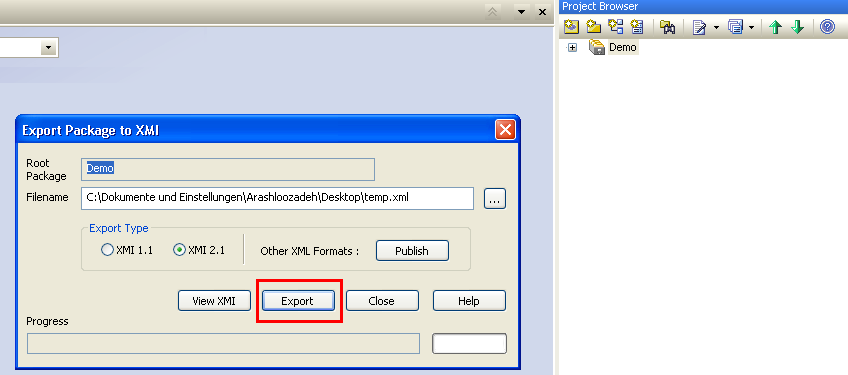
\includegraphics[width=0.5\textwidth]{pics/tricks/projectMigration/projectMigration2}
  \caption{Specify the Export file properties}  
  \label{fig_projectMigration02}
\end{center}
\end{figure}

\item[$\blacktriangleright$]In the next step you have to confirm importing of
XMI file(Fig.~\ref{fig_projectMigration05}).

\begin{figure}[htbp]
\begin{center}
  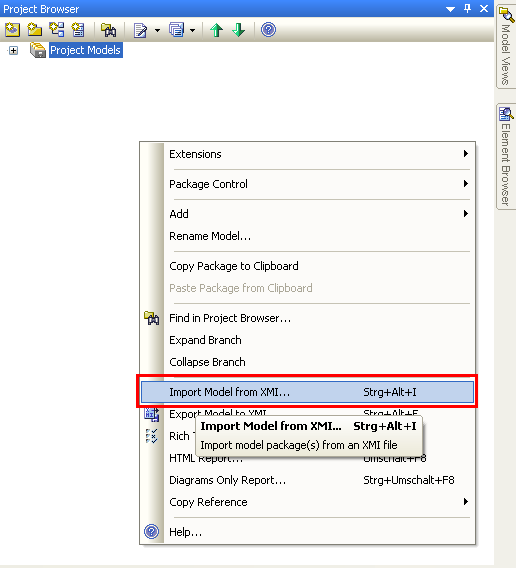
\includegraphics[width=0.5\textwidth]{pics/tricks/projectMigration/projectMigration3}
  \caption{Import the root node to the second EAP}  
  \label{fig_projectMigration03}
\end{center}
\end{figure}

\item[$\blacktriangleright$]Finally you have to specify the level of imported
file in the Project Browser either as Root Model or under selected
package (Fig.~\ref{fig_projectMigration06}).After Importing you have the whole root with all it's belonging
packages in the second EAP. Now you can delete the packages which you do not
need from the Root Model (Fig.~\ref{fig_projectMigration07}).

\begin{figure}[htbp]
\begin{center}
  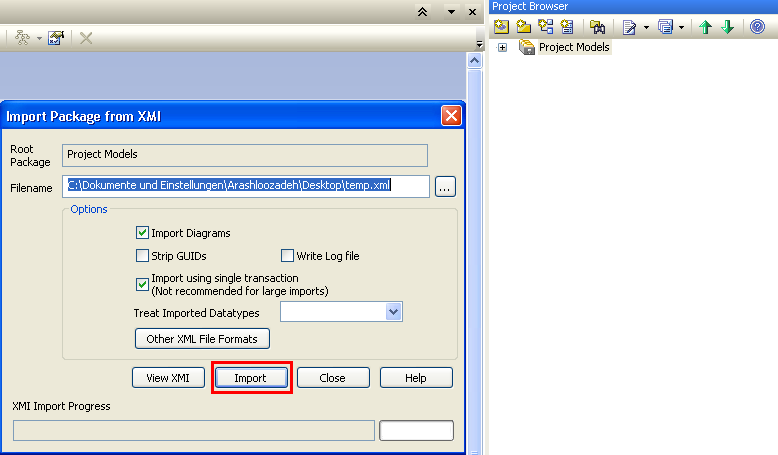
\includegraphics[width=0.5\textwidth]{pics/tricks/projectMigration/projectMigration4}
  \caption{Specify the Import file properties}  
  \label{fig_projectMigration04}
\end{center}
\end{figure}


\begin{figure}[htbp]
\begin{center}
  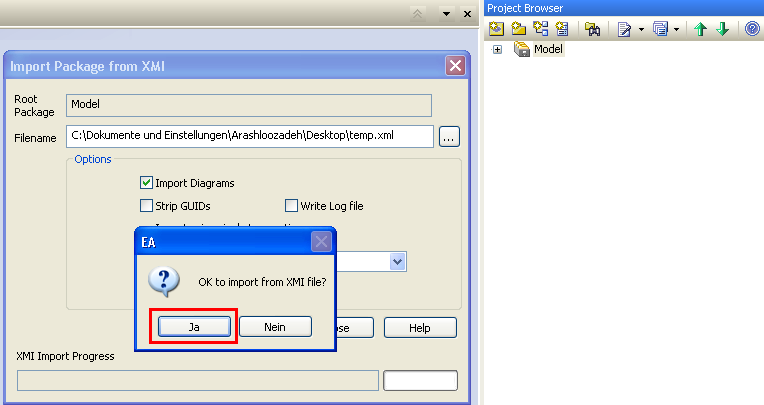
\includegraphics[width=0.5\textwidth]{pics/tricks/projectMigration/projectMigration5}
  \caption{Confirm Import}  
  \label{fig_projectMigration05}
\end{center}
\end{figure}



\begin{figure}[htbp]
\begin{center}
  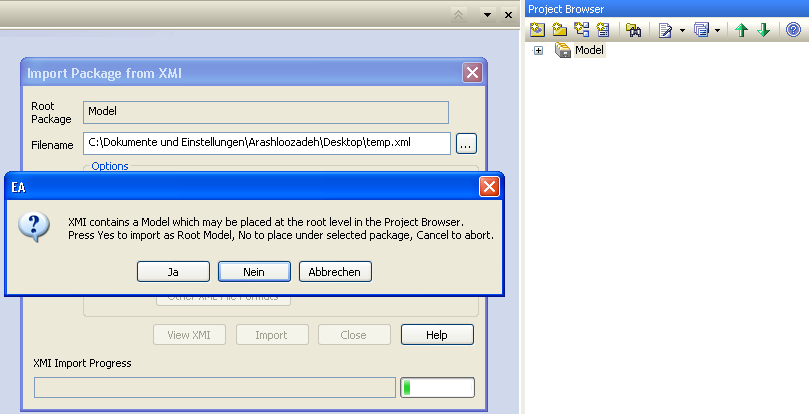
\includegraphics[width=0.5\textwidth]{pics/tricks/projectMigration/projectMigration6}
  \caption{Specify the level of imported model}  
  \label{fig_projectMigration06}
\end{center}
\end{figure}


\begin{figure}[htbp]
\begin{center}
  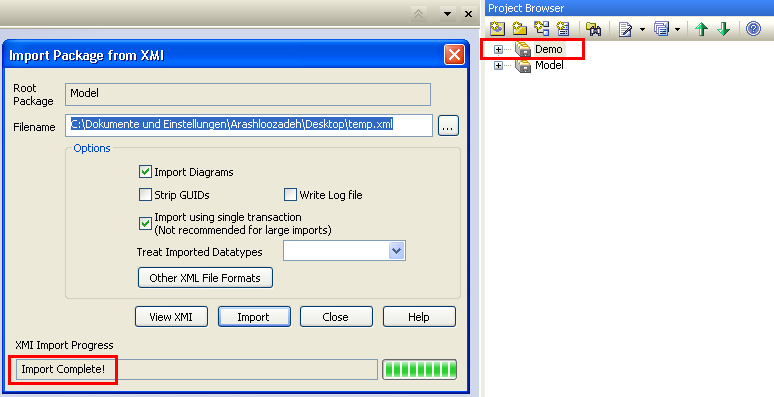
\includegraphics[width=0.5\textwidth]{pics/tricks/projectMigration/projectMigration7}
  \caption{Importing is completed}  
  \label{fig_projectMigration07}
\end{center}
\end{figure}


\end{enumerate}

